\chapter{Electric Fields}
\begin{itemize}
    \item \emph{Coulomb's Law} states that the \emph{magnitude} of the \emph{electric force} between two \emph{point charges} is directly proportional to the product of the charges, and inversely proportional to the square of their separation.
    \item The constant \(\varepsilon_0\) is the permittivity of \emph{free space} (\(\varepsilon_0\) is applicable only in air or a vacuum).
    \item Sign of \(F_E\):
    \begin{center}
        \begin{tabular}{|Sc|Sc|}
            \hline
            \(F_E\) & Direction\\
            \hline
            Positive & Repulsive\\
            \hline
            Negative & Attractive\\ 
            \hline
        \end{tabular}  
    \end{center}
    
  \item The sign of the electric force does \emph{not} represent the \emph{direction} of the electric force. It only informs us whether the force is attractive or repulsive. So, when calculating the \emph{resultant} electric force, we need to account for the direction ourselves. 
    \item Comparison between E-fields and G-fields: 
    \begin{center}
        \resizebox{0.942\textwidth}{!}{\begin{tabular}{|Sc|Sc|Sc|}
            \hline
            Sim/Diff & E-field & G-field\\
            \hline
            S & 
            \multicolumn{2}{Sc|}{\begin{minipage}{0.8\textwidth}
            For both Column's Law and Newton's Law of Gravitation, \(r\) is the \emph{center to center separation} of the objects.
            \end{minipage}}\\
            \hline
            S & 
            \multicolumn{2}{Sc|}{\begin{minipage}{0.8\textwidth}
            By Newton's Third Law, the \emph{forces} that masses and charges exert on each other is \emph{equal in magnitude} and \emph{opposite in direction}.
            \end{minipage}}\\
            \hline
            D & 
            \begin{minipage}{0.4\textwidth}
                Electric Forces can be \emph{attractive or repulsive}.
            \end{minipage} &
            \begin{minipage}{0.4\textwidth}
                Gravitational forces are \emph{always attractive}.
            \end{minipage}\\
            \hline 
    \end{tabular}}
    \end{center}
    \item An \emph{electric field} is a \emph{region in space} where a \emph{charge experiences an electric force}.
    \item How to draw electric field lines: 
    \begin{itemize}
        \item \emph{Lines cannot intersect} one another.
        \item Lines must \emph{begin from positive charges} and \emph{end on negative charges}.
        \item Arrows show the \emph{direction of force} exerted on a positive test charge.
        \item The \emph{greater} the electric field strength, the \emph{closer} together field lines are drawn.
        \item Lines leave/end on \emph{conducting surfaces} at \emph{right angles}
    \end{itemize}
    % POINT CHARGE +1
    \resizebox{0.942\textwidth}{!}{\begin{tikzpicture}
    \foreach \i [evaluate={\angle=(\i-1)*360/\NE;}] in {1,...,\NE}{
      \draw[EFieldLineArrow={0.6}] (0,0) -- (\angle:\R);
    }
    \draw[charge+] (0,0) circle (7pt) node[black,scale=0.8] {$+q$};
  \end{tikzpicture}
  % POINT CHARGE -1
  \begin{tikzpicture}
    \foreach \i [evaluate={\angle=(\i-1)*360/\NE;}] in {1,...,\NE}{
      \draw[EFieldLineArrow={0.5}] (\angle:\R) -- (0:0);
    }
    \draw[charge-] (0,0) circle (7pt) node[black,scale=0.8] {$-q$};
  \end{tikzpicture}
  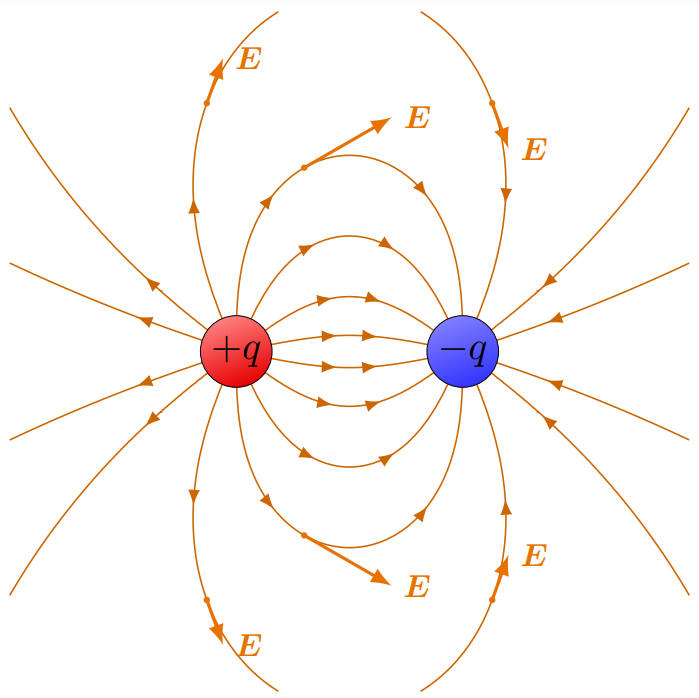
\includegraphics[width=0.25\textwidth]{../images/2 charges.png}
  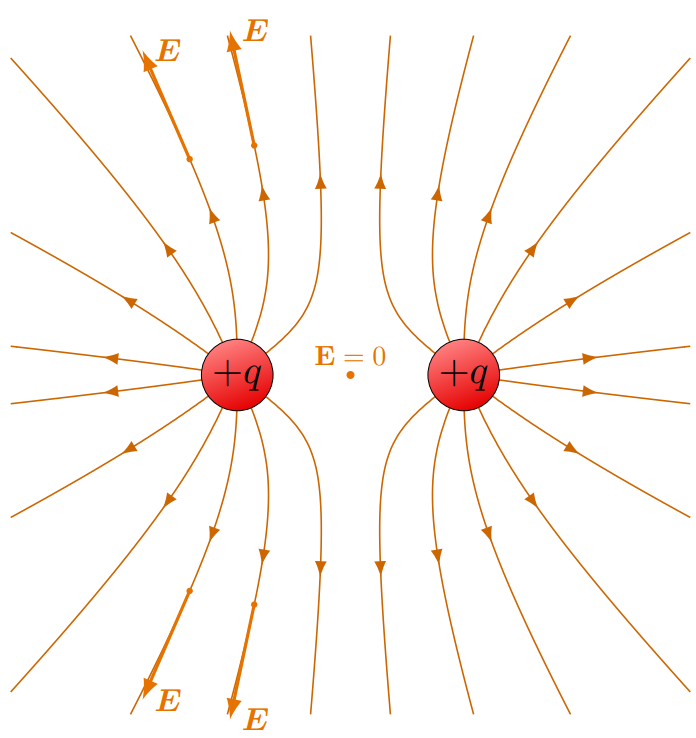
\includegraphics[width=0.25\textwidth]{../images/2repellingcharges.png}}
  \captionsetup{type=figure}
  \caption[figure]{\ref{Electric field lines of a point charge}, \ref{Electric field lines of two charges} Electric field lines of point charges and two interacting charges.}
  \begin{center}
    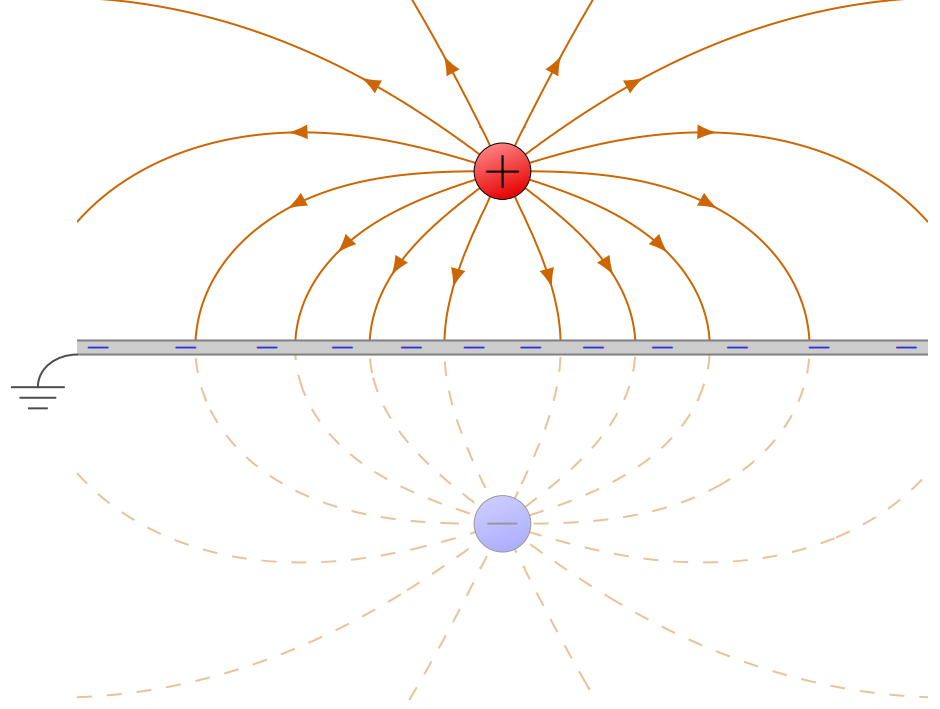
\includegraphics[width=0.5\textwidth]{../images/E-fieldPlate.png}
    \captionsetup{type=figure}
    \caption[figure]{\ref{Interaction of a point charge with a charged plate} Interaction of a point charge with a charged plate.}
  \end{center}
  \item The \emph{electric field strength} at a point is defined as the \emph{electric force} per \emph{unit positive charge} acting on a small stationary test charge placed at that point.
  \begin{center}
    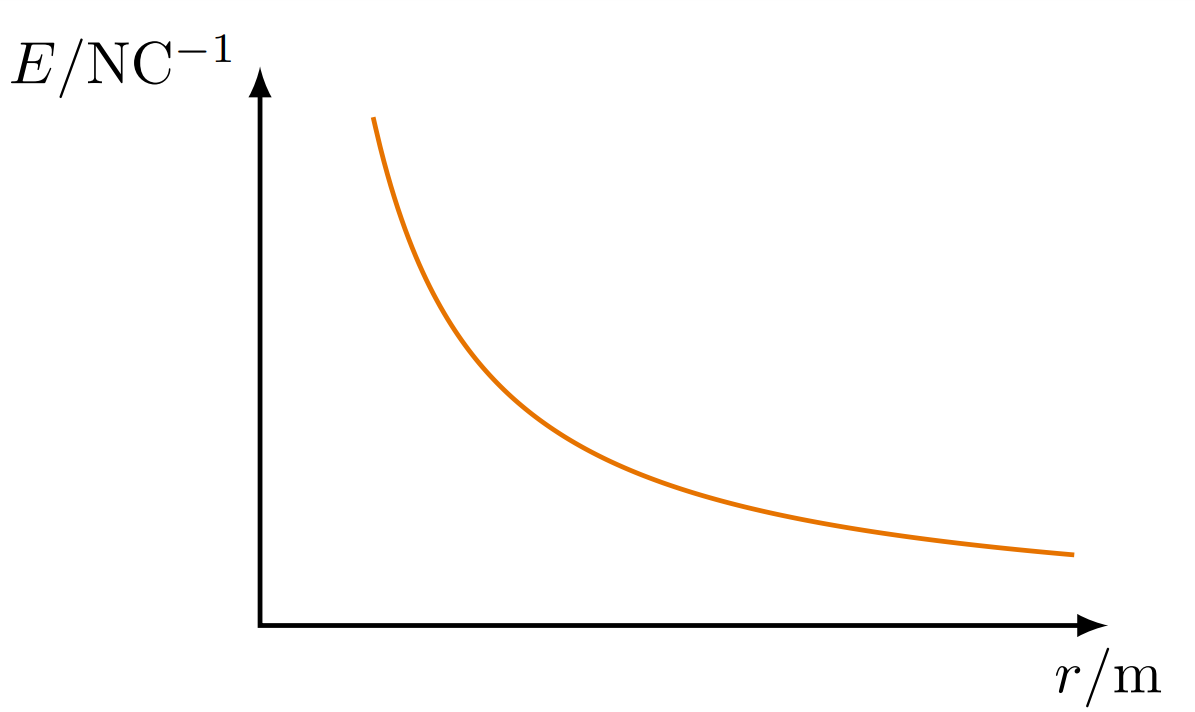
\includegraphics[width=0.5\textwidth]{../images/ElectricFieldStrengthPlot.png}
    \captionsetup{type=figure}
    \caption[figure]{\ref{Electric field plots} Electric field strength of a positive point charge}
  \end{center}
  \item The \emph{electric potential energy} of a point charge in an electric field is defined as the \emph{work done by an external agent} in bringing the point charge from infinity to that point (without any net change in kinetic energy). 
  \item The \emph{electric potential} at a point in an electric field is defined as the \emph{work done} per unit \emph{positive} charge, by an external agent, in bringing a \emph{small} test charge from infinity to that point (without any net change in kinetic energy). 
  \item Let \(U\) be the electric potential energy, and \(V\) the electric potential. Then,
  \[U=qV \qquad\text{and}\qquad \Delta U=q\Delta V.\]
  \begin{center}
    \begin{tikzcd}[row sep=large, column sep=large]
        U=\frac{Qq}{4\pi\varepsilon_0r} \arrow{r}{-\frac{\text{d}}{\text{d}r}} \arrow[swap]{d}{\frac{1}{q}} & F_E=\frac{Q_1Q_2}{4\pi\varepsilon_0r^2} \arrow[swap]{d}{\frac{1}{q}} \\
        V=\frac{Q}{4\pi\varepsilon_0r} \arrow{r}{-\frac{\text{d}}{\text{d}r}} & E=\frac{Q}{4\pi\varepsilon_0r^2}
    \end{tikzcd}
  \end{center}
  \item A ``singly charged'' object is one which has charge \(e=1.60\cdot 10^{-19}\). 
  \item The \emph{electric potential} at a point \(X\) due to a \emph{system} of point charges \(q_i\) is the algebraic sum of the electric potential \(V_i\) due to each individual charge \(q_i\) which is distance \(r_i\) away from \(X\). That is, 
  \[V=\sum_{i}{V_i}=\sum_{i}^{}{\frac{q_i}{4\pi\varepsilon_0r_i}}.\]
  \item The \emph{potential energy} of a \emph{system} of charges \(q_i\) is the work done to assemble it. This is the sum of energies \(U_{ij}\) needed to bring each charge \(q_i\) to the charges \(q_j\) (for \(i>j\)) already present. In other words letting \(r_{ij}\) be the distance of \(q_i\) from \(q_j\), we have 
  \[U=\sum_{i>j}{U_{ij}}=\sum_{i>j}^{}{\frac{q_iq_j}{4\pi\varepsilon_0r_{ij}}}.\] 
  \begin{figure}[H]
    \centering
    \begin{subfigure}{0.45\textwidth}
        \centering
        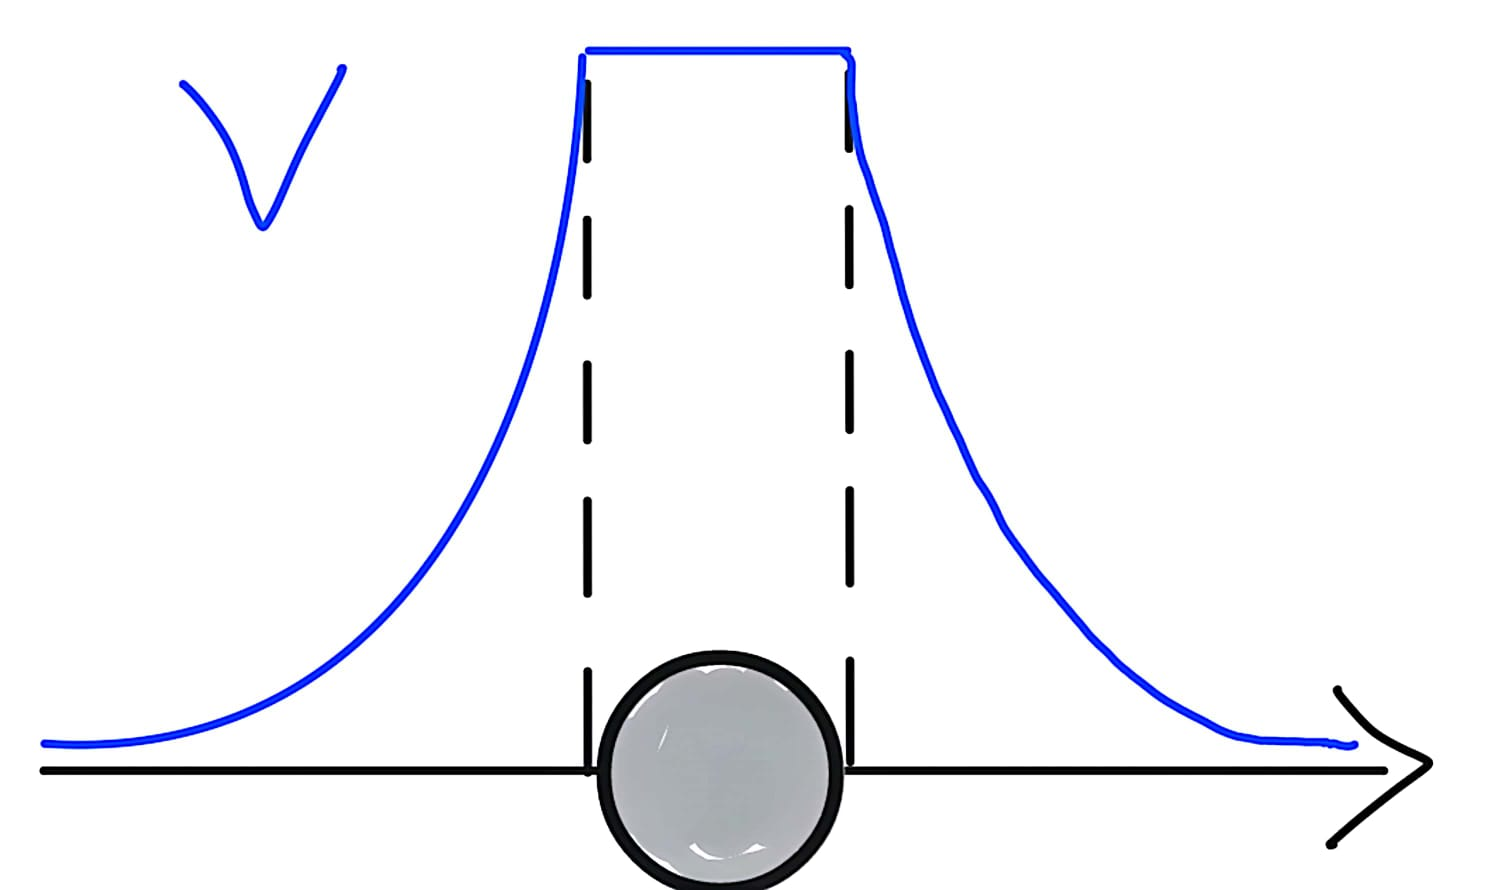
\includegraphics[width=\textwidth]{../images/Isolated Conductor/Potential.jpg}
        \caption{Potential.}
        \label{fig:isolated-conductor-potential}
    \end{subfigure}\hfill
    \begin{subfigure}{0.45\textwidth}
        \centering
        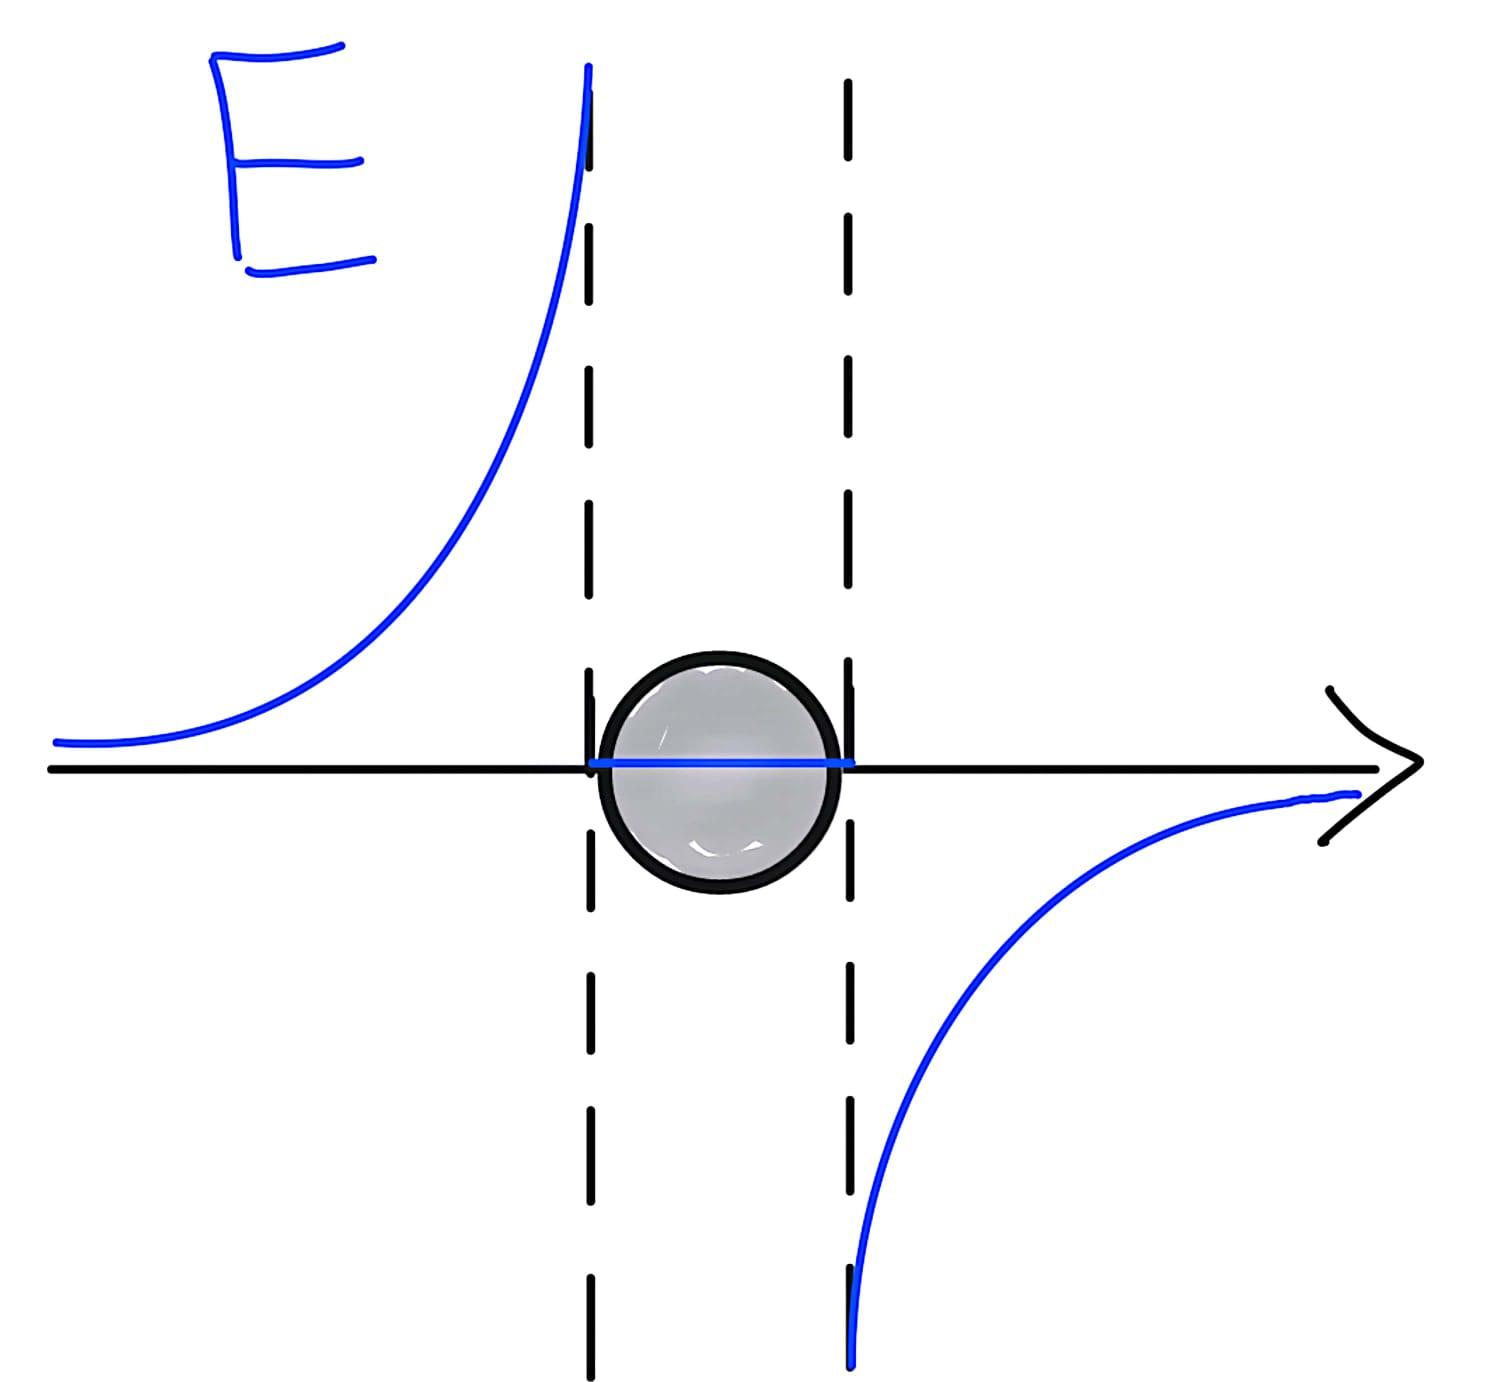
\includegraphics[width=\textwidth]{../images/Isolated Conductor/Electric field strength.jpg}
        \caption{Field strength.}
        \label{fig:isolated-conductor-field-strength}
    \end{subfigure}
    \caption{The electric potential and electric field strength around an isolated conductor.}
    \label{fig:isolated-conductor}
\end{figure}
  \item Charge distribution on a conducting sphere: 
  \begin{itemize}
    \item Excess charges are forced to the surface of the conductor until the electric field inside the conductor is zero. 
    \item \emph{Outside} the conductor, the electric field is the \emph{same} as that of an isolated point charge equal to the excess charge. 
  \end{itemize}
  \item Properties of conductors in \emph{electrostatic equilibrium}:
  \begin{itemize}
    \item The \emph{electric field is zero inside} a conductor (regardless of shape).
    \item So, the \emph{entire conductor} is at the \emph{same potential}.
    \item Just outside the conductor, the e-field lines are \emph{perpendicular to its surface}, starting and ending on charges on the surface.
    \item \emph{Excess charges} resides exclusively on \emph{the surfaces} of a conductor.
  \end{itemize}
  \item Electric field strength between two charged parallel plates is uniform everywhere between the plates, except at both ends of the plates. 
  \item Also, \emph{charges} between the plates experience \emph{uniform acceleration}.
  \begin{center}
    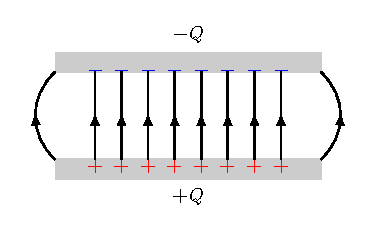
\includegraphics[scale=1]{../images/ParallelPlates/testing.pdf}
    \captionsetup{type=figure}
    \caption[figure]{\ref{Electric field lines between parallel plates} Electric field lines between parallel plates.}
  \end{center}
  \item Magnitude of electric field strength between the plates:
  \[E=\frac{dV}{dr}=\frac{\Delta V}{d}.\]
\end{itemize}
\begin{figure}[H]
    \centering
    \begin{subfigure}{0.4\textwidth}
        \centering
        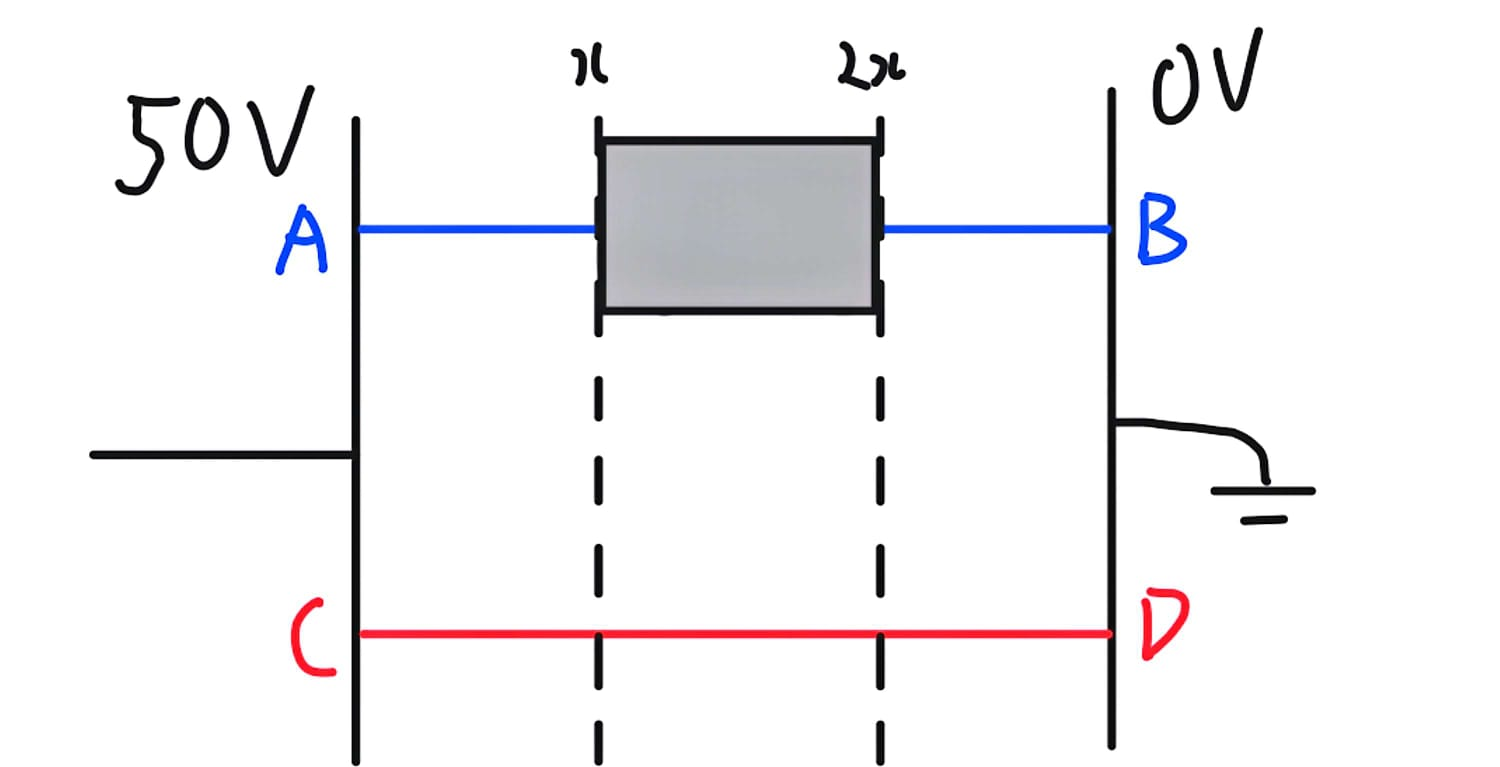
\includegraphics[width=\textwidth]{../images/Electric Conductor/Setup.jpg}
        \caption{The setup.}
        \label{fig:electric-conductor-plot-setup}
    \end{subfigure}\hfill
    \begin{subfigure}{0.3\textwidth}
        \centering
        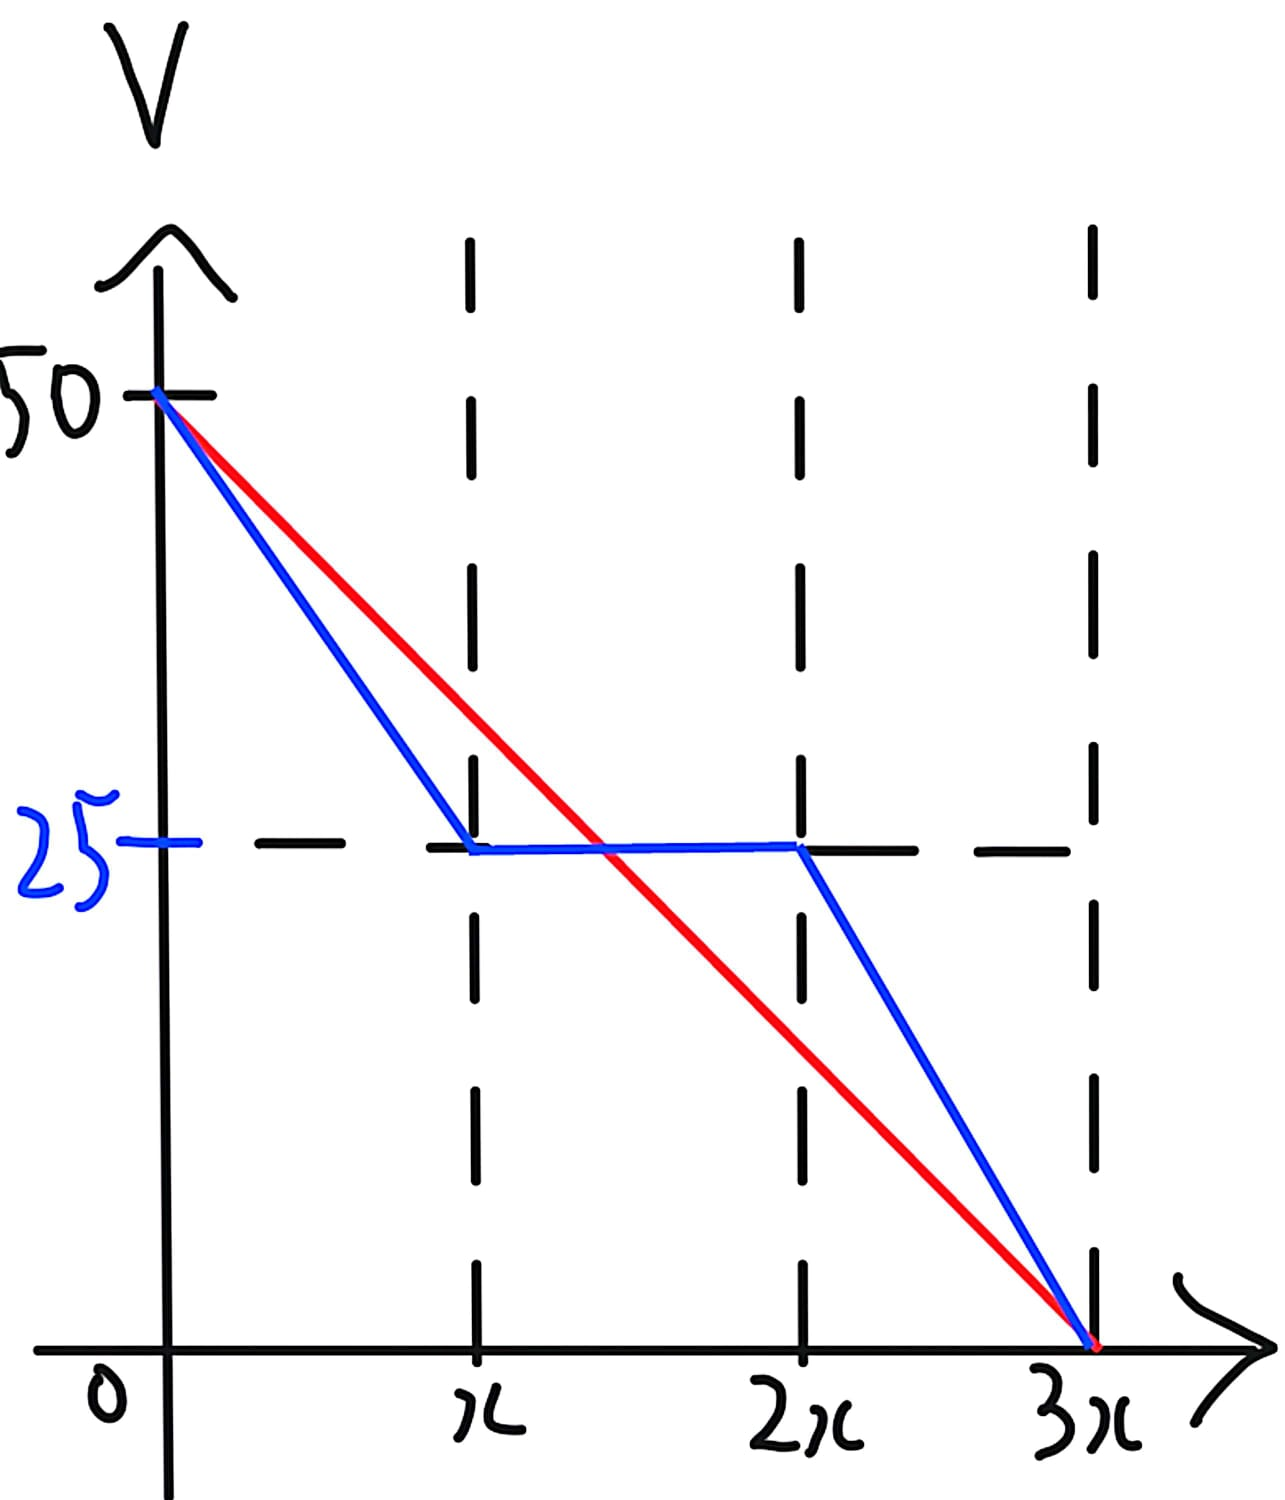
\includegraphics[width=\textwidth]{../images/Electric Conductor/Potential.jpg}
        \caption{Potential.}
        \label{fig:electric-conductor-plot-potential}
    \end{subfigure}\hfill
    \begin{subfigure}{0.3\textwidth}
        \centering
        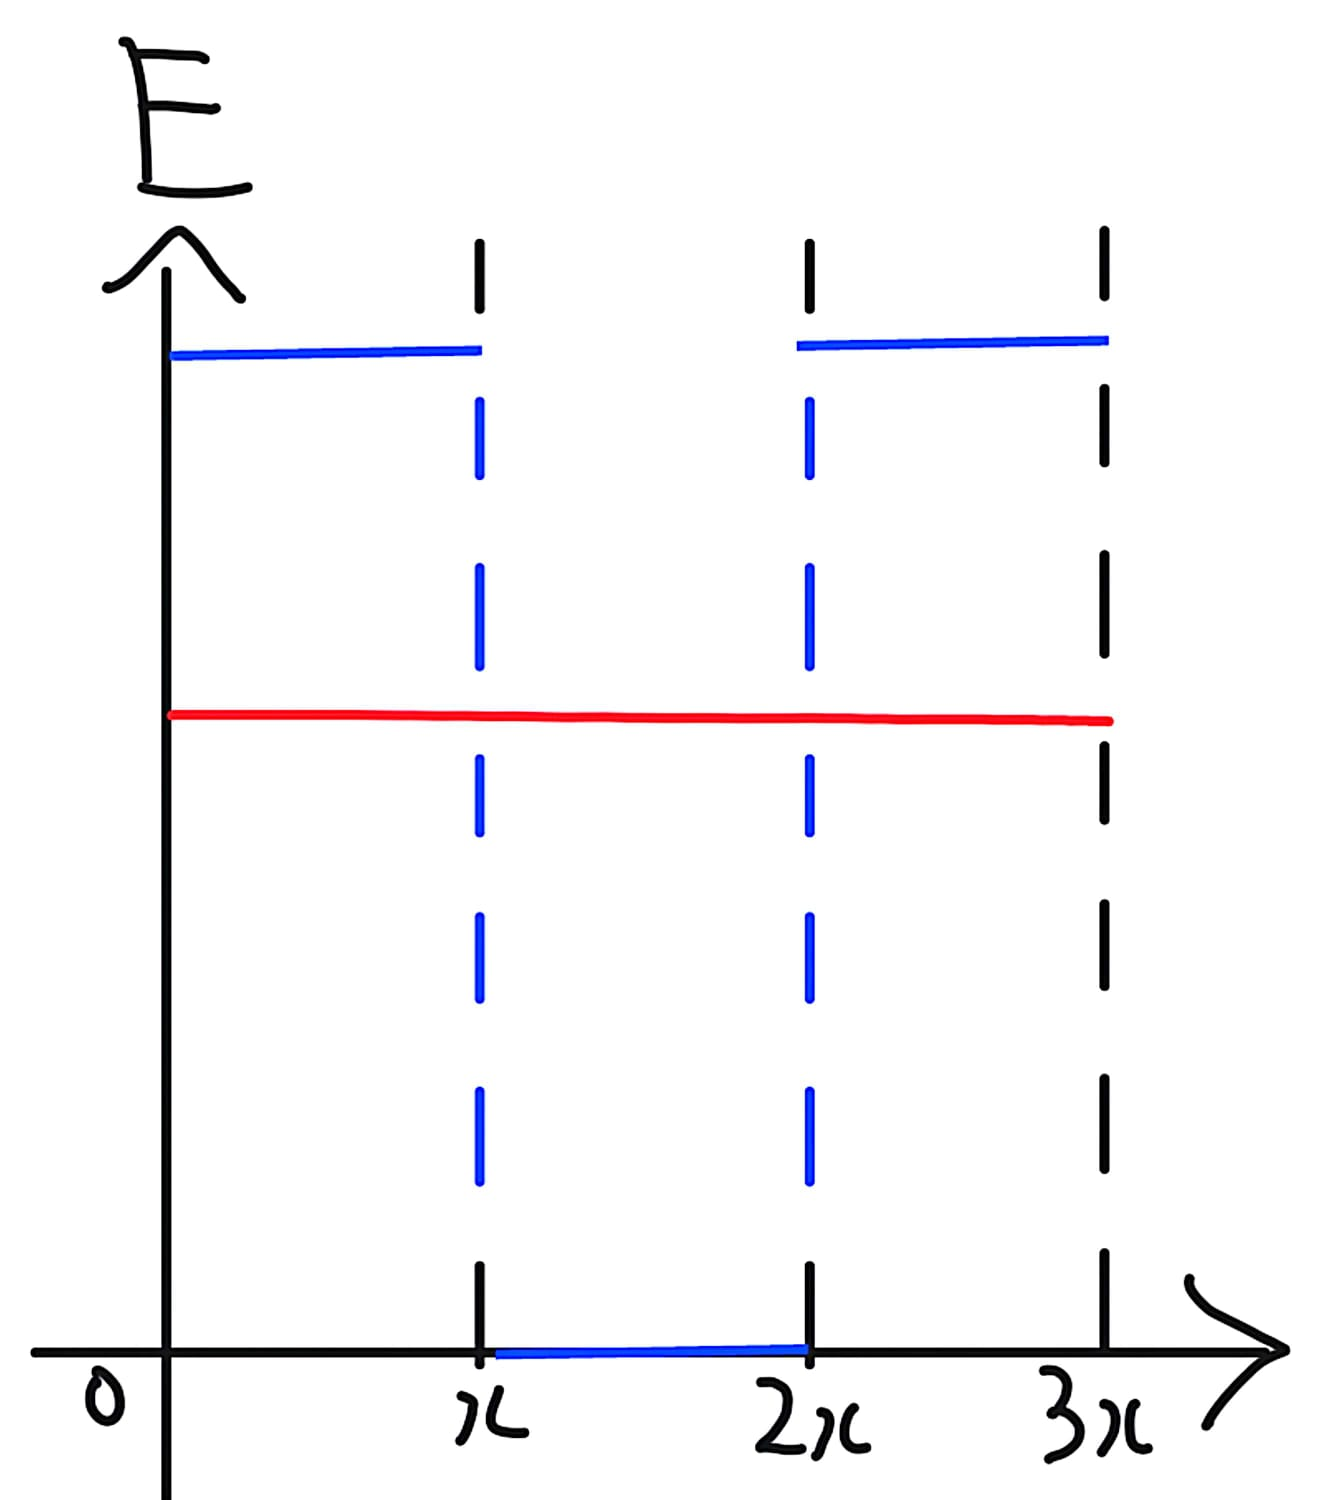
\includegraphics[width=\textwidth]{../images/Electric Conductor/Field Strength.jpg}
        \caption{Field strength.}
        \label{fig:electric-conductor-plot-field-strength}
    \end{subfigure}
    \caption{The electric potential and electric field strength between two parallel plates containing a conductor.}
    \label{fig:electric-conductor-plot}
  \end{figure}
  \begin{example}{}{}
    \begin{figure}[H]
        \centering
        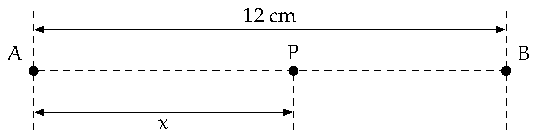
\includegraphics{../images/electric-charge-sign-from-graph/setup.pdf}
        \caption{\ref{Me} Two point charges, \(A\) and \(B\), are separated in a vacuum by a distance of 12cm.}
        \label{fig:two-point-charges-setup}
    \end{figure}
    \begin{figure}[H]
        \centering
        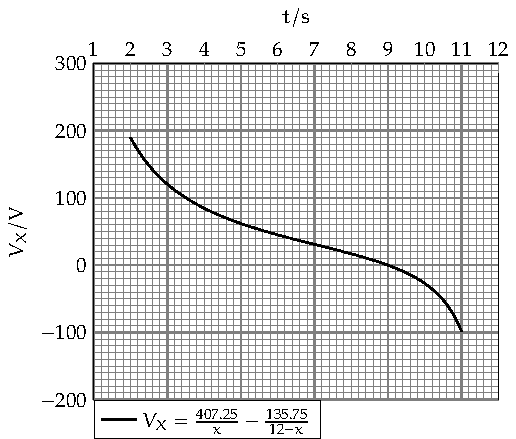
\includegraphics{../images/electric-charge-sign-from-graph/electric-potential-graph.pdf}
        \caption{\ref{Me} The variation with distance \(x\) of the electric potential \(V_X\) at point \(P\).}
        \label{fig:net-electric-potential-due-to-two-point-charges}
    \end{figure}
    Explain whether the charges have the same, or opposite, signs.
    \begin{itemize}
        \item The potential due to two charges at a point is the scalar sum of the potentials due to each charge at the same point.\footnote{This point can be skipped, if the question is one mark and time is running short.}
        \item Since potential is positive near to \(A\) and negative close near to \(B\), charges \(A\) and \(B\) are positive and negative, respectively.
        \item i.e. the charges have opposite signs.
    \end{itemize}
  \end{example}
\begin{center}
    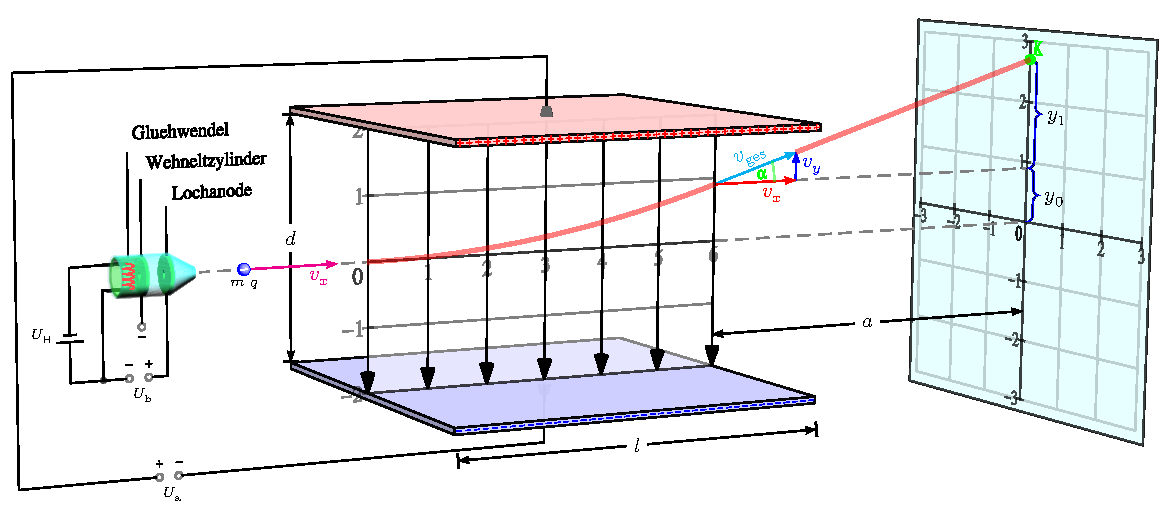
\includegraphics[width=\textwidth]{../images/Electron-Deflection/Bahn-Kondensator (1).pdf}
    \captionsetup{type=figure}
    \caption[figure]{\ref{Electron deflection} Deflection of an electron.}
\end{center}